\subsection{Distinguishing correction from smoothing}
\label{sec:result-corr_smooth}


A possible objection to the decrease in footprint RMSE result of Sect.~\ref{sec:result-tccon_val} is that the \emph{DE} model may act as a local low-pass filter. Since the near-cloud bias appears as short-scale structure along the orbit, any procedure that averages neighboring footprints would also collapse the within-overpass scatter, and the station-day comparison might not distinguish the two. To test this possibility directly, we construct a feature-free smoother null and evaluate it with exactly the same footprints, output guards, and AK-harmonized TCCON chain as the production correction.

For footprint $i$, the smoothed product is the orbit-local running mean of the operational product,
%
\begin{equation}
  X^{\mathrm{sm}(W)}_{\mathrm{CO2},i}
  = \frac{1}{\left|\mathcal{N}_i(W)\right|}
    \sum_{j \in \mathcal{N}_i(W)} X^{\mathrm{B11}}_{\mathrm{CO2},j},
  \qquad
  \mathcal{N}_i(W)
  = \left\{\, j \;:\; \left|t_j - t_i\right| \le W \,\right\},
  \label{eq:smoother}
\end{equation}
%
where $t_i$ is the sounding time and $\mathcal{N}_i(W)$ is restricted to the same contiguous along-track segment (a time gap larger than 30~s starts a new segment) and the same surface type as footprint $i$, mirroring the per-surface construction of the model; the footprint itself is included in the mean, as for any symmetric smoother. The implied pseudo-correction is $\mu^{\mathrm{sm}}_i = X^{\mathrm{B11}}_{\mathrm{CO2},i} - X^{\mathrm{sm}(W)}_{\mathrm{CO2},i}$, which replaces the deep-ensemble $\mu_i$ in the evaluation chain. We test half-widths $W = 10$, 30, and 100~s, corresponding to roughly $\pm 67$, $\pm 200$, and $\pm 675$~km along track. The smoother uses no predictor features and no cloud information: it is the strongest form of the ``the correction only smooths'' hypothesis.

The two diagnostics separate cleanly (Fig.~\ref{fig:smoother_null}). On the within-overpass footprint scatter, the smoother is stronger than the \emph{DE} model as expected. The per-case mean scatter falls from 2.23~ppm to 0.66, 0.51, and 0.35~ppm for $W = 10$, 30, and 100~s, compared with 0.78~ppm for the deep ensemble. A running mean minimizes local variance by construction, so on this metric alone the null cannot be rejected. The station-day mean $|$bias$|$ to TCCON, however, is left essentially unmoved by the smoother: 1.26~ppm before correction against 1.24, 1.20, and 1.20~ppm after smoothing, whereas the deep ensemble reduces it to 0.82~ppm. The reason is structural: because the running mean approximately preserves the overpass-mean \xco, it can only redistribute the error among footprints, not remove it, while the deep ensemble shifts the mean itself. We conclude that variance removal alone cannot reproduce the observed bias reduction, and that the validation improvement of Sect.~4.4 reflects a genuine correction of the near-cloud bias rather than local denoising. Figure~\ref{fig:smoother_null} shows the $W = 30$~s arm; the $\pm 10$ and $\pm 100$~s arms behave the same way and are given in Appendix~\ref{app:null-test} (Fig.~\ref{app-fig:smoother_null_full}).




The smoother collapses footprint scatter more strongly than the \emph{DE} model (0.35–0.66 vs 0.78 ppm) yet leaves the TCCON station-day mean $|$bias$|$ essentially unmoved (1.20–1.24 ppm, against 0.82 ppm for the model). In other words, variance removal alone cannot produce the observed bias reduction, and the correction by the \emph{DE} model reduces both observed bias and spread.




\begin{figure}[t]
\centering
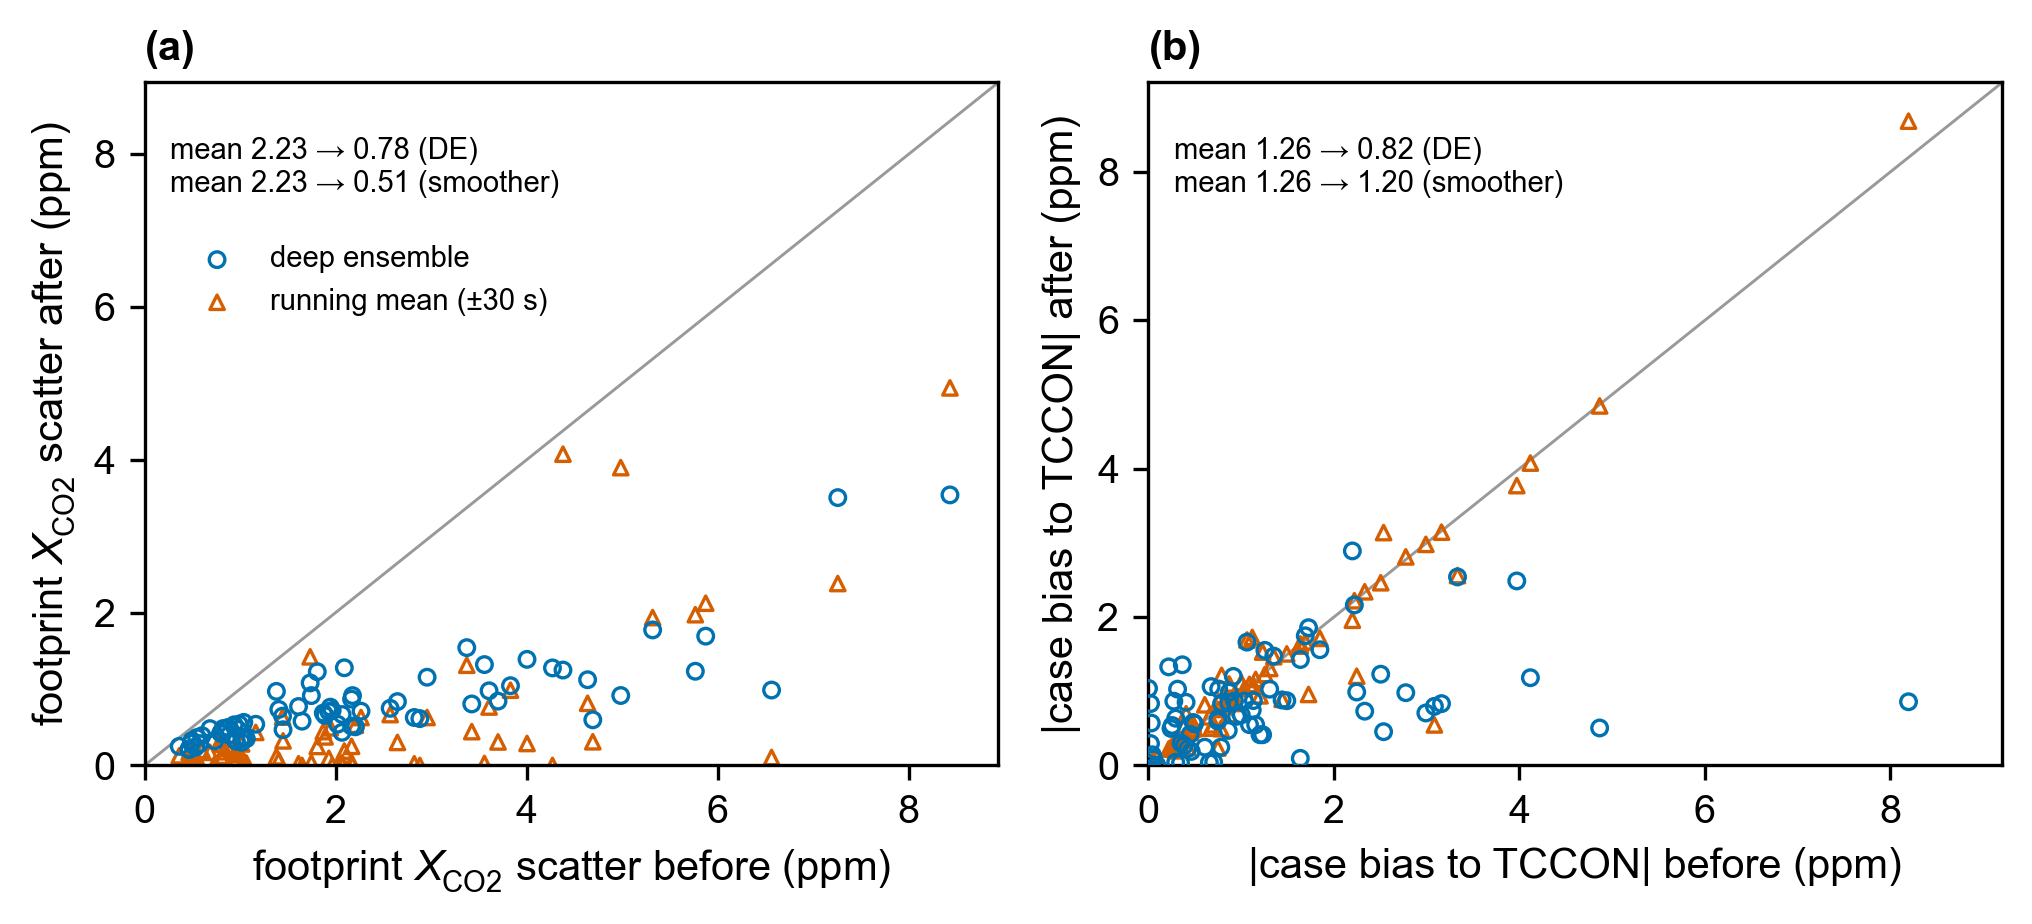
\includegraphics[width=0.8\textwidth]{figures/fig10_smoother_null.png}
\caption{Correction versus smoothing null test. A feature-free orbit-local running-mean smoother (±10/30/100 s half-widths, screened by the same input guards as the production correction) compared with the deep ensemble on footprint scatter (a) and TCCON station-day mean $|$bias$|$ (b).}
\label{fig:smoother_null}
\end{figure}



\FloatBarrier